\documentclass[11pt, twocolumn]{article}
\usepackage{geometry}                % See geometry.pdf to learn the layout options. There are lots.
\geometry{letterpaper}                   % ... or a4paper or a5paper or ... 
%\geometry{landscape}                % Activate for for rotated page geometry
%\usepackage[parfill]{parskip}    % Activate to begin paragraphs with an empty line rather than an indent
\usepackage{graphicx}
\usepackage{amssymb}
\usepackage{amsmath}
\usepackage{epstopdf}
% Package for including code in the document
\usepackage{listings}
\usepackage{fullpage}


\DeclareGraphicsRule{.tif}{png}{.png}{`convert #1 `dirname #1`/`basename #1 .tif`.png}



\title{PCA Analysis using Core Image}
\author{Daniel Beatty}

%\date{2007-05-05}
%\date{}                                           % Activate to display a given date or no date

\begin{document}
\maketitle
%\section{}
%\subsection{}




\section{Introduction}

The core essence of Principle Component Analysis is in finding a set of orthogonal basis vectors for a collection of vectors assembled in a matrix.  Such a basis allows the original data to mapped into this orthogonal space.  There are well studied methods for obtaining principle components such as Karhunen-Loeve and Singular Value Decomposition.  While it is true that they each obtain equivalent results, how they do it determines their effectiveness at achieving these results.  Also, some methods have side-products which may be useful.  

In the end, the principle components are simply defined in terms of eigenvectors and their eigenvalues for a ``scatter'' matrix.  These vectors happen to belong to the columns of the $V$ matrix of the SVD $\mathbf{A} = \mathbf{U\Lambda V}^T$.  Likewise, the eigenvalues of the scatter matrix are part of the diagonal matrix $\Lambda$.  Since the SVD was part of the LAPACK wrappers of the dcgRenaissance, this logical choice of implementation for acquiring the SVD.  

This experiments original instructions was to use Principal Component Analysis (PCA) in combination with the Whitening transform and Linear Discriminant Analysis (LDA) to classify and segment the optic disc from the background.   The PCA by itself is not a classifier.  Rather it finds orthogonal vectors that a representative of the data.  Applying the principle components to the data simply transforms the data into another orthogonal space.  Also, Fisher's Linear/Multiple Discriminant Analysis depends on previous samples for each desired class.   

For demonstration purposes, the points in question are preselected on a pixel coordinate system.  The pixels for each class are therefore used in determining the LDA.  Accuracy of the LDA does have some dependency on the quality of the samples chosen.  The chosen test image happens to be a classic image of a human optic disc.  Fortunately, the disc is in the center of the image.  Thus one choice for member of the disc would be all pixels in a radius of 25 pixels from the center.  Pixels close to borders of the image are definitely not part of the optic disc.  Thus we have a collection samples to call our class samples.  

It it were not for this convenient example, a more elaborate interface would be required to identify samples belong to specific classes.  This is useful in an application, but not a unit test type experiment.  Such region of interest exercises, even with Core Image, are deemed beyond the scope of this exercise.  

%Also, this allow for more complex parameters to be considered.  Parameters could include the gradient(s) of points, averages of points, and image transformations placed matrix where the row vectors contained points and their neighbors for each of processed image type.  
Many parameters may be considered for PCA.  A single point itself is not particularly interesting, as such an eigenvector would be a scalar.  However, neighborhoods of both the image itself, and transformations such a gradients, edge transformations, and others tend to be quite interesting for this experiment.  

The neighborhood concept comes from digital image processing techniques of segmentation called Local Processing Edge Linking and Boundary Detection.   In this technique, boundaries are determined by the image's gradient in row wise, column wise, and in some cases diagonal wise.  From any of these, a set of row vectors may be formed consisting the values for the point itself in both the original image and resulting images from the application of gradient and other operators.  In addition the row vector can include neighborhood values, differences, angles, and angle differences.  At which point one has a substantial set of parameters to categorize any point.  The use of PCA allows these parameters to be mapped to an orthogonal space, which in some cases allows simplified categorization.  


In this case, we are using 5 by 5 neighborhoods of the gradient differences, angle differences, the original image neighborhood, and gradient row and column neighborhoods.   While this is certainly excessive, it does allow for a demonstration.   

\section{Unit Test of PCA}
The experiment requested for this project is significantly more complex than what a unit test should test.  Any unit test should have a simple input, simple output, and known comparison for the output.   An example of this would be say a matrix 

\begin{eqnarray}
\mathbf{A}= 
\left\{
\begin{array}{llll}
1	& 	2 	& 	3	& 	4 \\
5	&	6	& 	7	& 	8 \\
9	&	10	&	11	&	12 \\
13	&	14	&	15	&	16 \\
\end{array}
\right\} \\
\mathbf{U} = 
\left\{
\begin{array}{llll}
-0.13		& 0.82	& -0.54	& 0.03 \\
-0.34 	& 0.42	&  0.75	& 0.36	\\
-0.54		& 0.03	& 0.13	& -0.8	\\
-0.75		& -0.36	& -0.341	& 0.42
\end{array}
\right\} \\
\mathbf{\Lambda}
\left\{
\begin{array}{llll}
38	& 0. 		& 0. 	&  0.\\
0.		& 2.07	& 0.	& 0.\\
0.		& 0.		& 0.	& 0.\\
0.		& 0.		& 0.	& 0.
\end{array}
\right\} \\
\mathbf{V}^T =
\left\{
\begin{array}{llll}
-0.42		& -0.71	& -0.16	& -0.52	\\
-0.47		& -0.27	& 0.60	& 0.57	\\
-0.52		& 0.17	& -0.72	& 0.41	\\
-0.56		& 0.61	& 0.28	& -0.47
\end{array}
\right\} \\
\textrm{SVD} (\mathbf{A}) = U \Lambda V^T \\
V = \textrm{eigenvectos}(\mathbf{A}\mathbf{A}^T) \\
\Lambda = \textrm{eigenvalues}(\mathbf{A}\mathbf{A}^T) 
\end{eqnarray}
The values for $\mathbf{U}$, $\mathbf{\Lambda}$, and $\mathbf{V}$. are computed using Mathematica's pre-canned Singular Value Decomposition method.   A comparison between this and the unit test can be valuable. 
%Of course, Mathematica has pre-canned variety of the SVD, and we can simply use it to provide quickly a result can compare it to the results of the unit test.   

Similarly, the results from the MDA assignment using Mathematica can be used as a unit test for the LDA/ MDA component.  The results are expected to be similar, within a scaling factor.  

\section{Interface design}
In order to complete the assignment, a tool is necessary that uses this build framework, identifies the regions of interest for the MDA/LDA preprocessing,  and neighborhoods, and use these libraries to produce the principle components.    The results from the preprocess operations need to be fed into a mask generating classifier.  

\begin{figure}[htbp] %  figure placement: here, top, bottom, or page
   \centering
   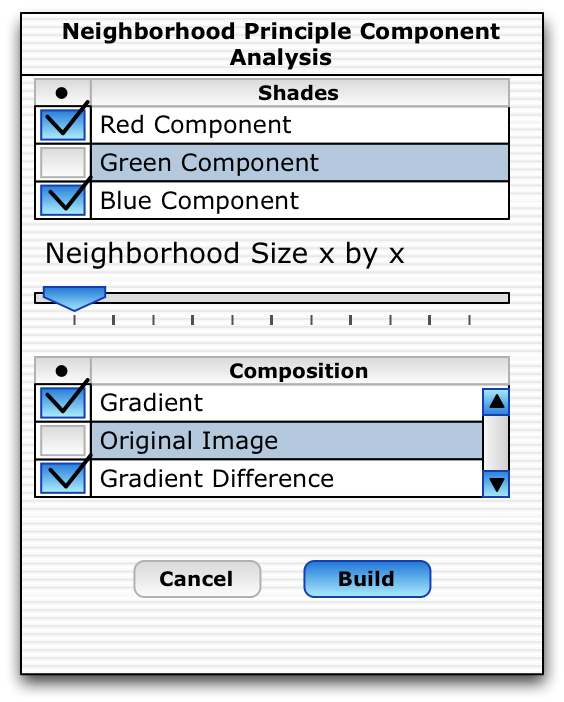
\includegraphics[width=3in]{neighborhoodPCA.png} 
   \caption{This panel selects the neighborhood, and components to use.}
   \label{neighborhoodPCA}
\end{figure}


\begin{figure}[htbp] %  figure placement: here, top, bottom, or page
   \centering
   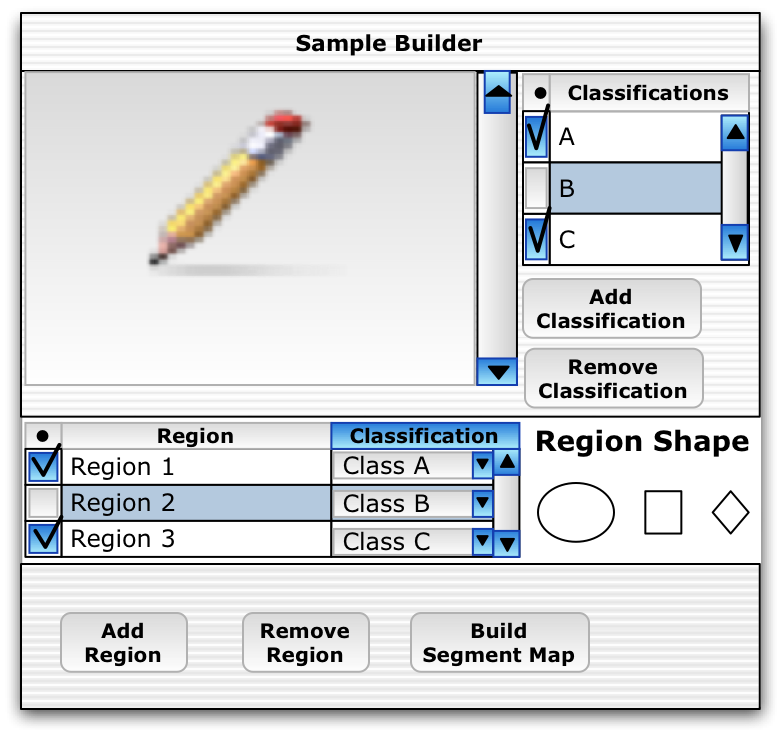
\includegraphics[width=3in]{regionOfInterestPanel.png} 
   \caption{This panel selects the regions of interest, and instructs the building of classes.}
   \label{regionOfInterestPanel}
\end{figure}

\begin{figure}[htbp] %  figure placement: here, top, bottom, or page
   \centering
   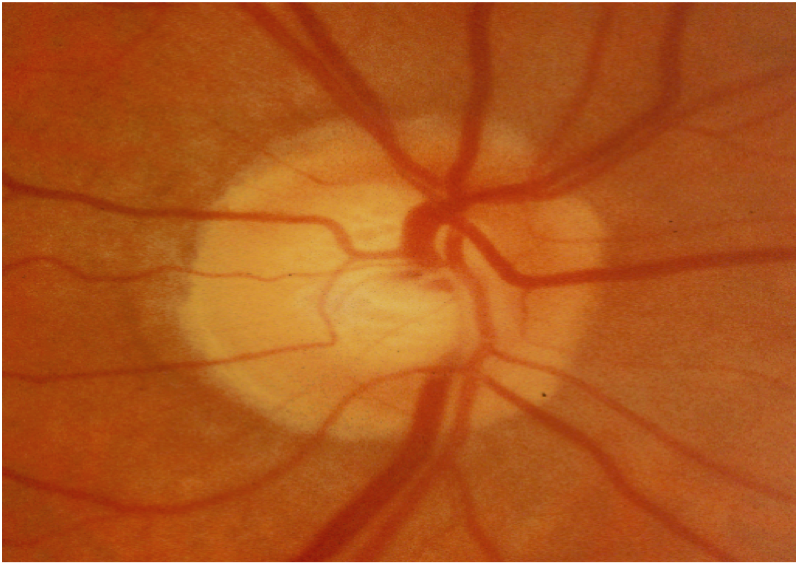
\includegraphics[width=3in]{opticDisc.png} 
   \caption{Original image of the optic disc of a human eye.}
   \label{originalOpticDisc}
\end{figure}


\begin{figure}[htbp] %  figure placement: here, top, bottom, or page
   \centering
   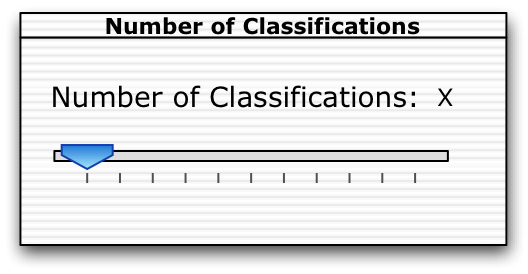
\includegraphics[width=3in]{numberOfClassificationsSlider.png} 
   \caption{Slider panel for specifying the number of classifications.}
   \label{numberOfClassificationsSlider}
\end{figure}

\begin{figure}[htbp] %  figure placement: here, top, bottom, or page
   \centering
   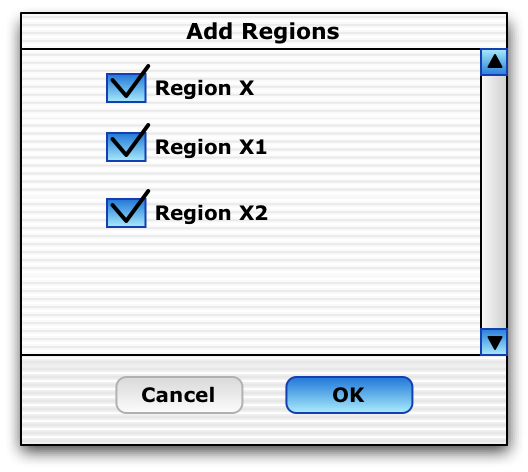
\includegraphics[width=3in]{addRegionsCheckBoxes.png} 
   \caption{Table for selecting regions to add to a classification.}
   \label{addRegionsCheckBoxes}
\end{figure}

numberOfClassificationsSlider

Region of Interest Control:
\begin{itemize}
	\item List Control
\end{itemize}

Non-kernel based Region of Interest View applies to a view that displays both the image and boxes identifying regions of interest.  A region of interest contains points known to belong to a classification.
\begin{itemize}
	\item ROIView $\to$ OpenGLView?  QuartzView?
	\item Initialize called by either the opening of a nib file or object initialization.
	\begin{itemize}
		\item ``initWithFrame''
		\item ``awakeFromNib''
	\end{itemize}
	\item Drawing methods \\
	drawRect
	\item What do we need:
	\begin{itemize}
		\item Need ability to identify selected ROI.
		\item Overrides on mouse and arrow.
	\end{itemize}
	
\end{itemize}


Mask Selection:
\begin{itemize}
	\item Selection of masks (maskControl)
\end{itemize}

Neighborhood Builder
\begin{itemize}
	\item Size
	\item Component
	\item Composition
	\begin{itemize}
		\item gradient
		\item Original Image
		\item Gradient difference
		\item Gradient Angle
		\item Gradient Angle Difference
	\end{itemize}
	
\end{itemize}


Neighborhood Control
\begin{itemize}
	\item Component List
	\item (Action) Construct Neighborhoods
\end{itemize}

Bayes Gaussian Multivariate Control Control
\begin{itemize}
	\item Multivariate Classes
	\item Classifier List
	\begin{itemize}
		\item Name
		\item Member regions
		\item (Action) add classification
		\item (Action) add region to classification.
	\end{itemize}
	
\end{itemize}

\bibliography{../../patternNotes.bib}

\bibliographystyle{abbrv}

\end{document}  

